Aplikacja konsolowa powstała w celu przetwarzania czasochłonnych zadań w tle, tak by użytkownik aplikacji webowej nie doświadczał długich czasów ładowania oraz ewentualnych błędów podczas przerwania sesji lub połączenia internetowego ze stroną. Aplikacja konsolowa uruchamiana jest co 5 minut i przetwarza zadania trzech typów w kolejności widocznej na rysunku \ref{fig:worker_proces}. Poszczególne procesy zostały szerzej opisane w kolejnych podrozdziałach.
\begin{figure}[H]
	\centering
	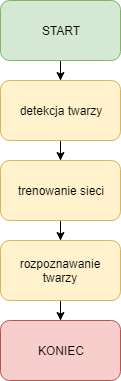
\includegraphics[scale=0.6]{worker_proces.png}
	\caption{Proces działania aplikacji konsolowej}
	\label{fig:worker_proces}
\end{figure}

\section{Technologie}
Aplikacja konsolowa powstała w języku programowania Python w wersji trzeciej. W początkowej fazie projektu za wyborem tego języka przemawiała wieloplatformowość, możliwości wprowadzania szybkich zmian w kodzie i brak potrzeby go kompilowania. C\#, który został wybrany do stworzenia aplikacji webowej okazał się nie przystosowany do uruchomienia na platformie Raspberry Pi z powodu braku dostępnego .NET Core SDK na procesory ARM oraz wymaganiu znacznie większej ilości zasobów niż Python. Ostatecznie aplikacja konsolowa została przeniesiona na zewnętrzny serwer, ale popularność Pythona pozwoliła na szybką integrację z usługami firm trzecich, dzięki przygotowanym przez firmy paczki deweloperskie.

\section{Proces wykrywania twarzy}
Uogólniony proces detekcji twarzy na obrazie został przedstawiony na grafie \ref{fig:wykrywanie_proces}.
Proces przetwarzania zadań detekcji rozpoczyna się od pobrania z bazy wszystkich żądań o statusie 'New'. Następnie każde zadanie przetwarzane jest osobno. Dla aktualnie procesowanego zadania pobierany jest obraz wejściowy z usługi Dropbox i zapisywany w lokalnym folderze. Następnym krokiem jest wywołanie procesu odpowiedzialnego za odpowiednie przygotowanie zdjęcia, a następnie pozyskanie oczekiwanych wyników, w sposób odpowiedni dla danego sposobu. Krok ten został szerzej opisany w rozdziale \ref{detekcja_twarzy}. po uzyskaniu wyników każdą dostępną w programie metodą, zostaje utworzony obraz wyjściowy dla każdej metody (haar, azure, ..), które zostaje zuploadowany do odpowiedniego folderu na Dropboxie oraz dodany do relacyjnej bazy danych MSSQL. Po wykonaniu zadania bez żadnych błędów, request zostaje oznaczony jako zakończony, w innym przypadku zostaje nadany mu status 'Error'. Proces powtarzany jest dla każdego wpisu pozyskanego z bazy.
\begin{figure}[H]
	\centering
	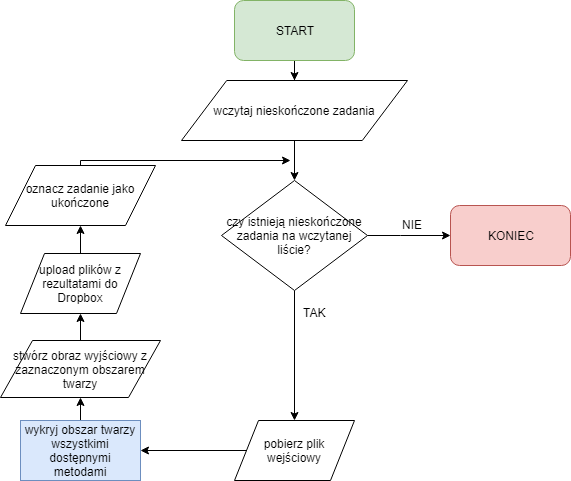
\includegraphics[scale=0.6]{wykrywanie_twarzy.png}
	\caption{Proces wykrywania twarzy}
	\label{fig:wykrywanie_proces}
\end{figure}

\subsection{Open Cv Haar}
\begin{figure}[H]
	\centering
	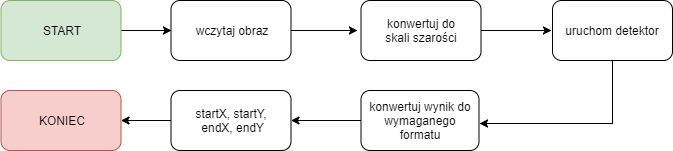
\includegraphics[scale=0.6]{detekcja_haar.png}
	\caption{Proces trenowania sieci}
	\label{fig:trenowanie_proces}
\end{figure}

\subsection{Open Cv Dnn}
\begin{figure}[H]
	\centering
	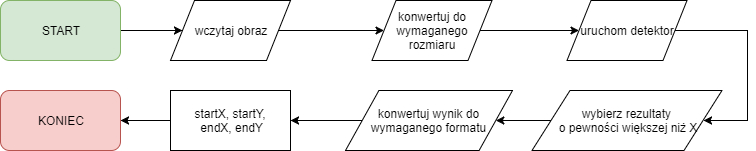
\includegraphics[scale=0.6]{detekcja_dnn.png}
	\caption{Proces trenowania sieci}
	\label{fig:trenowanie_proces}
\end{figure}

\subsection{Azure Cognitive Services}
\begin{figure}[H]
	\centering
	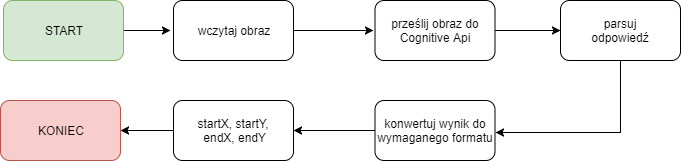
\includegraphics[scale=0.6]{detekcja_azure.png}
	\caption{Proces trenowania sieci}
	\label{fig:trenowanie_proces}
\end{figure}


\section{Proces trenowania sieci neuronowych}
Proces trenowania sieci został przedstawiony na grafie \ref{fig:trenowanie_proces}. Proces zaczyna się od sprawdzenia jakie dane uczące (osoby utworzone w zakładce 'People' aplikacji webowej) są dostępne lokalnie. Repozytorium zostaje porównane z danymi dostępny w bazie, a następnie zostają pobrane zdjęcia wszytskich brakujących osób do lokalnej ścieżki. Kolejnym krokiem jest pobrania z bazy wszystkich nowych grup sieci neuronowych, które nie zostały jeszcze zakończone. Następnie dla każdego zgłoszenia z listy wykonywany jest proces przygotowania danych uczących na podstawie zdjęć osób, które wybrano podczas tworzenia sieci neuronowej w aplikacji webowej. Po odpowiednim przygotowaniu danych sieć zostaje nauczona i dla większości metod zostaje utworzony plik w formacie xml przechowujący wytrenowany model. Taki plik zostaje dodany do bazy oraz wysłany do odpowiedniego folderu w Dropboxie. W przypadku braku komplikacji, request zostaje oznaczony jako zakończony. Proces zostaje powtórzony dla każdego zadania wczytanego do listy na początku grafu. Sposób przygotowania danych oraz nauczania dla poszczególnych metod został opisany w kolejnych podrozdziałach.
\begin{figure}[H]
	\centering
	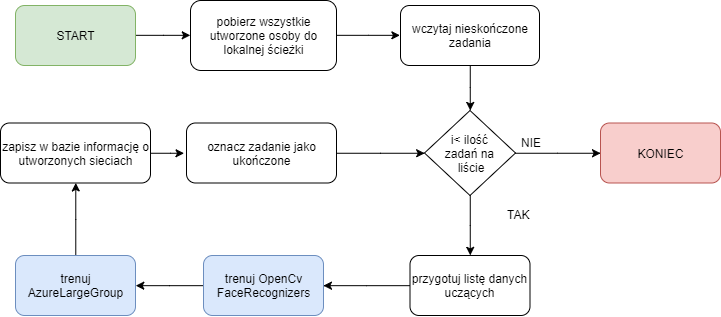
\includegraphics[scale=0.6]{proces_nauczania.png}
	\caption{Proces trenowania sieci}
	\label{fig:trenowanie_proces}
\end{figure}

\subsection{Trenowanie identyfikatorów Open Cv} \label{trenowanie_open_cv}

\begin{figure}[H]
	\centering
	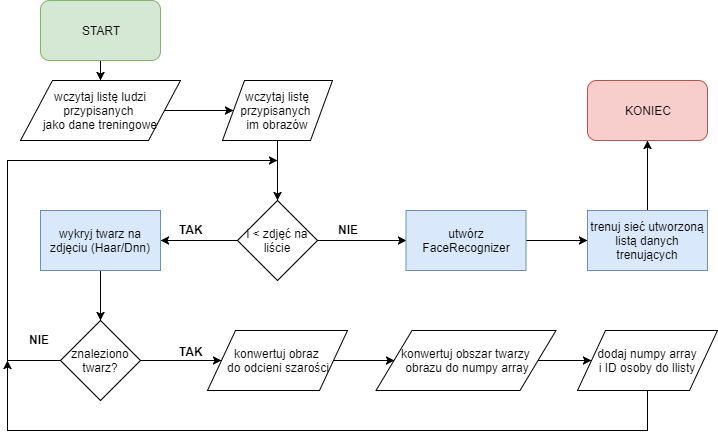
\includegraphics[scale=0.6]{trenowanie_open_cv.png}
	\caption{Trenowanie sieci neuronowej Open Cv}
	\label{fig:trenowanie_open_cv}
\end{figure}

\subsection{Trenowanie identyfikatora Azure} \label{trenowanie_open_cv}
\begin{figure}[H]
	\centering
	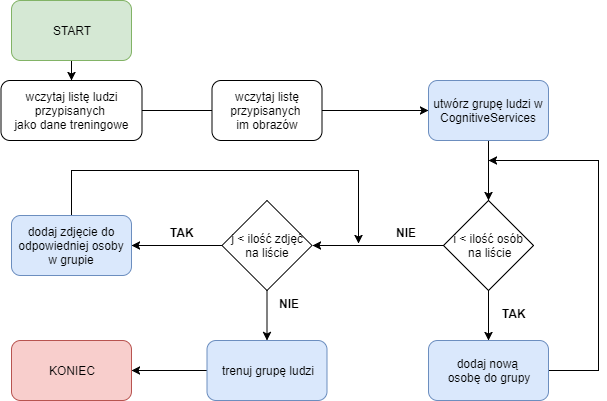
\includegraphics[scale=0.6]{trenowanie_azure.png}
	\caption{Trenowanie sieci neuronowej usługi Azure Cognitive Services}
	\label{fig:trenowanie_azure}
\end{figure}

\section{Proces rozpoznawania twarzy}
\begin{figure}[H]
	\centering
	\includegraphics[scale=0.6]{rozpoznawanie_twarzy.png}
	\caption{Proces identyfikacji tożsamości}
	\label{fig:rozpoznawanie_proces}
\end{figure}

\subsection{OpenCv}
\begin{figure}[H]
	\centering
	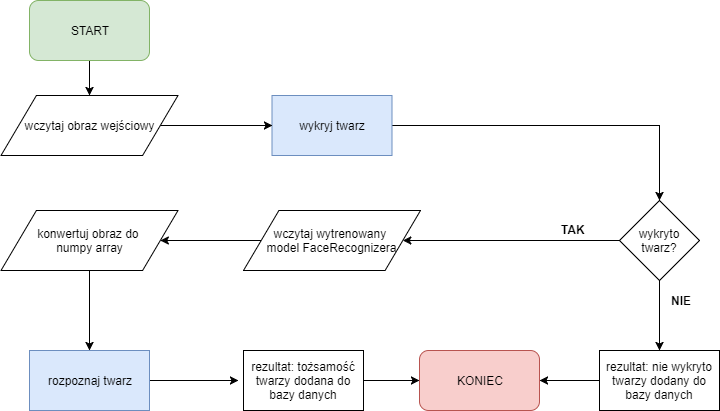
\includegraphics[scale=0.6]{rozpoznawanie_open_cv.png}
	\caption{Proces identyfikacji osoby wykorzystując Open Cv}
	\label{fig:rozpoznawanie_open_cv}
\end{figure}

\subsection{Azure Cognitive Services}
\begin{figure}[H]
	\centering
	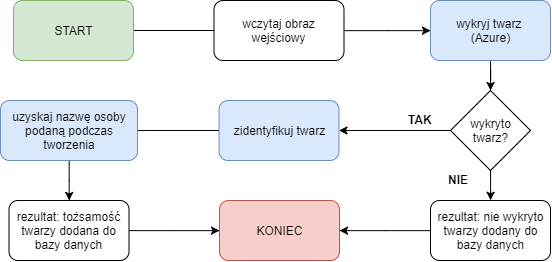
\includegraphics[scale=0.6]{rozpoznawanie_azure.png}
	\caption{Proces identyfikacji osoby wykorzystując Azure Cognitive Servces}
	\label{fig:rozpoznawanie_open_cv}
\end{figure}